% Example template for using the unmeethesis style
% This example is for a Master's candidate in Mathematics
% It contains examples of front matter and most sections that the
% typical graduate student would need to include
% By: N. Doren 02/10/00
%     Minor mods by N. Doren 08/26/11

% Use the following specification for BOTTOM page numbering:
\documentclass[botnum, fleqn]{unmeethesis}
\usepackage{amssymb}

\usepackage{bm}
\usepackage{graphicx}
\usepackage{float}
\usepackage{amsmath}
\usepackage{ amssymb }
                 % OR
% Use the following specification for TOP page numbering:
% \documentclass[fleqn]{unmeethesis}

\begin{document}

\frontmatter


% Uncomment the next command if you see weird paragraph spacing:
% That is, if you see paragraphs float with lots of white space
% in between them:

% \setlength{\parskip}{0.30cm}


\title{Optimal Transport Driven Bayesian Inversion with Application to Signal Processing}

\author{Elijah Perez}

\degreesubject{M.S., Mathematics}

\degree{Master of Science \\ Mathematics}

\documenttype{Thesis}

\previousdegrees{B.S., Mathemtics, University of New Mexico, 2019}

\date{July, \thisyear}

\maketitle

%\makecopyright
%Copyright page is no longer necessary D. Murrell

\begin{dedication}
   To my parents, Phillip and Martha, and my wife, Jessica. For their love and support. \\[3ex]
   ``If I have seen further it is by standing on the shoulders of Giants.''
         -- Isaac Newton
\end{dedication}

%\begin{acknowledgments}
%   \vspace{1.1in}
%   I would like to thank my advisor, Professor Martin Sheen, for his support
%   and some great action movies.  I would also like to thank my dog, Spot,
%   who only ate my homework two or three times.  I have several other people
%   I would like to thank, as well.\footnote{To my brother and sister, who
%   are really cool.}
%\end{acknowledgments}

\maketitleabstract %(required even though there's no abstract title anymore)

\begin{abstract}
   This paper will outline a Debiased Sinkhorn Divergence driven Bayesian inversion framework. Conventionally, a Gaussian Driven Bayesian framework is used when performing Bayesian inversion. A major issue with this Gaussian framework is that the Gaussian likelihood, driven by the $L_2$ norm, is not affected by phase shift in a given signal. This issue has been addressed in [1] using a Wasserstein framework. However, the Wasserstein framework still has an issue because it assumes statistical independence when multidimensional signals are analyzed. This assumption of statistical independence cannot always be made when analyzing signals where multiple detectors are recording one event, say from a seismic event. The Wasserstein metric can be generalized to multidimensional signals, but implementation of the multidimensional Wasserstein metric is very computationally expensive. This means that it is unreasonable for Bayesian inversion. Debiased Sinkhorn Divergence offers an alternative to the multidimensional Wasserstein metric while remaining relatively cheap computationally. This allows for the creation of a Debiased Sinkhorn Divergence driven Bayesian framework that will be formulated and analyzed in this paper.
\clearpage %(required for 1-page abstract)
\end{abstract}

\tableofcontents
\listoffigures
%\listoftables

%\begin{glossary}{Longest  string}
%   \item[$a_{lm}$]
%      Taylor series coefficients, where $l,m = \{0..2\}$
%   \item[$A_{\bf{p}}$]
%      Complex-valued scalar denoting the amplitude and phase.
%   \item[$A^T$]
%      Transpose of some relativity matrix.
%\end{glossary}

\mainmatter

\chapter{Introduction}
%\section{\label{section:overview}Overview}
   In most applications of Bayesian inversion, a Gaussian likelihood (sometimes called Normal likelihood) function is used to formulate a Bayesian inversion framework. The Gaussian likelihood implements the $L_2$ norm. This likelihood function is a standard choice in certain specific applications, but fails to account for phase differences in a given signal. Because of this, the Gaussian likelihood can produce many false optima that a Bayesian inversion algorithm can become trapped in, producing an incorrect posterior distribution. Through the work in [1] we can see that a way to avoid this issue all together is to use a different likelihood, namely a quadratic Wasserstein quasi-likelihood (loss function). The advantage that this quasi-likelihood has is that the Wasserstein metric not only measures the difference in amplitude of two signals, but also the difference in phase. This means that depending on the application, the Wasserstein quasi-likelihood can produce a better posterior compared to the Gaussian likelihood. This idea is explored in detail in [1]. The Wasserstein metric is used to create the Wasserstein quasi-likelihood and in [1], the one-dimensional Wasserstein metric is used. This is because implementation of a multidimensional Wasserstein metric would be very computationally expensive. So, instead of implementing the multidimensional Wasserstein metric, [1] uses the one-dimensional Wasserstein metric and makes some assumptions on the signal being analyzed. The main assumption is that the signals being analyzed are statistically independent. This assumption is made so that we can assume that the quasi-likelihood of the signals is a product of the quasi-likelihoods of the one-dimensional signals. This assumption allows the one-dimensional Wasserstein quasi-likelihood to be applied to multidimensional signals. However, this assumption of statistical independence cannot always be made for a given set of signals. This is where Debiased Sinkhorn Divergence has a major advantage. Sinkhorn Divergence can be viewed as an entropically regularized Wasserstein distance[2][17], allowing for the creation of a Debiased Sinkhorn Divergence driven Bayesian framework. This Sinkhorn framework has the advantage that it does not require the assumption of statistical independence to work. Sinkhorn has an advantage over the multidimensional Wasserstein metric in that it is far less computationally expensive [18]. Because Sinkhorn Divergence costs less computationally than the multidimensional Wasserstein metric, it is a viable option in a Bayesian framework. Also, Sinkhorn Divergence does not need the statistical independence assumption, so it can be a better choice when analyzing a multidimensional signal compared to the one-dimensional Wasserstein metric. In this paper a Sinkhorn Divergence Bayesian framework is created by modifying the Wasserstein framework from [1], using a Markov Chain Monte Carlo method. Specifically, Metropolis-Hastings within Gibbs sampling algorithm will be used to formulate a numerical algorithm (see chapter 5 for details). \\
   The rest of the paper will explore this new Sinkhorn-Bayesian framework. Chapter 2 will outline the general Bayesian inversion Problem. Chapter 3 will explore how to derive Sinkhorn divergence from the general optimal transport problem. Chapter 4 will outline quasi-likelihood structures based on Sinkhorn and Wasserstein. Chapter 5 will describe a numerical method using the new Sinkhorn quasi-likelihood. Chapter 6 will explore examples implementing this new Sinkhorn-Bayesian framework. 
   
%\section{Conclusions}
%   I conclude that this is a really short thesis.

\chapter{Bayesian Inversion}
\section{\label{section:Bayes' Theorem}Bayes' Theorem}
In many stochastic processes, we are tasked with finding the conditional probability of the model parameter given an observed quantity. This is done through Bayes’ Theorem which allows us to calculate the conditional probability of an event occurring. In Bayesian inversion, we are using Bayes’ Theorem to calculate the conditional probability of the model parameter vector $\bm{\theta} = (\theta_1, ..., \theta_m) \in \Theta \subset \mathbb{R}^m $. Let $\bm{g}=(g_1,…,g_n) \in \mathbb{R}^n$ be vector of $n$ observed quantities and let $\bm{f}=(f_1,…,f_n) \in \mathbb{R}^n$ be a vector of $n$ predicted quantities created by a forward predictive model depending on the parameter vector $\bm{\theta}$. That is: 
\begin{center}
$\bm{f}=\bm{f}(\bm{\theta}): \Theta \subset \mathbb{R}^m \rightarrow \mathbb{R}^n$ 
\end{center}
Now, applying Bayes’ Theorem to solve for the conditional probability of $\bm{\theta}$ given $\bm{g}$, written as $\pi(\bm{\theta}|\bm{g})$, we have [3]:


	\hspace{\fill}$\pi(\bm{\theta}|\bm{g})=$\Large$\frac{\pi(\bm{g}|\bm{\theta})\pi(\bm{\theta})}{\int_{\Theta}\pi(\bm{g}|\bm{\theta})\pi(\bm{\theta})d\bm{\theta}}$ \hspace{\fill} \normalsize (1) 

	

\noindent Where $\pi(\bm{\theta}|\bm{g})$ is the posterior, $\pi(\bm{g}|\bm{\theta})$ is the likelihood, and $\pi(\bm{\theta})$ is the prior distribution of $\bm{\theta}$. Note that sometimes $\int_{\Theta}\pi(\bm{g}|\bm{\theta})\pi(\bm{\theta})d\bm{\theta}$ is written as $\pi(\bm{g})$. Since $\pi(\bm{g})$ is independent of $\bm{\theta}$, it can be viewed as a scaling constant to ensure that the posterior obtained from (1) is consistent with the definition of a probability density function (i.e. $\int_{\Theta}\pi(\bm{\theta}|\bm{g})d\theta=1$ and is positive for $\forall \bm{\theta} \in \Theta$). This means that $\pi(\bm{\theta}|\bm{g}) \propto \pi(\bm{g}|\bm{\theta})\pi(\bm{\theta})$, and that the proportionality constant is precisely {\large$\frac{1}{\pi(\bm{g})}$}. This now leaves the task of finding distributions for the prior and likelihood. The prior, $\pi(\bm{\theta})$, is a distribution that we obtain from prior knowledge about the model parameter $\bm{\theta}$. As an example, if we know that $\bm{\theta} \in(1,3)$ then one choice for a prior could be $\bm{\theta}\sim Uniform(1,3)$. \\\\Now, if we have a quasi-likelihood instead of a true likelihood, we call the resulting posterior distribution a quasi-posterior or Gibbs posterior. This Gibbs posterior still gives accurate information on the probability of $\bm{\theta}$ given $\bm{g}$, but is defined using a quasi-likelihood and thus cannot be called a true posterior [22]. These quasi-likelihoods are defined by loss functions and still give information about goodness of fit, and can be a more realistic choice in Bayesian processes because the true underlying likelihood function may be unknown. This means that the Gibbs posterior results in near identical results to the true posterior, while offering a more general framework that works for applications for which the true likelihood function is unknown [22] (see section 6.2 and Figure 6.2). 
\section{\label{section:Likelihood Structure}Likelihood Structure}
The choice of likelihood is a fundamental step in Bayesian inversion and is one of the main aspects of Bayesian inversion that can be changed. Often, the choice of a likelihood function is based on the noise structure that the analyzed signal is expected to have. Under the assumption that we have a simple additive noise structure, the Gaussian likelihood is the most common choice. Assuming that we have measurement noise $(\epsilon_1,…,\epsilon_n)$ that appears in the measured quantities $(g_1,…,g_n)$ the additive noise is assumed to be normally distributed with mean zero and standard deviation $\sigma$. That is to say:
\begin{center}
$g_i=f_i(\bm{\theta})+\epsilon_i$,\hspace{1cm} $\epsilon_i\sim Normal(0, \sigma)$,\hspace{1cm} $i=1,…,n$
\end{center}
Where $n$ is the number of measured quantities. This noise structure can be handled well by the Gaussian likelihood [1]:

\hspace{\fill}	$L_{norm}(\bm{\theta})=\pi_{norm}(\bm{g}|\bm{\theta})=$ \large$\frac{1}{(2\pi)^{n/2}\sigma^n}$\normalsize exp$(\frac{-1}{2\sigma^2}\sum_{i=1}^{n}|g_i-f_i(\bm{\theta})|^2)$\hspace{\fill} \normalsize (2)

Such a likelihood structure also requires an assumption of statistical independence for the signals being analyzed. This is seen in the fact that the overall likelihood, $\pi(\bm{g}|\bm{\theta})$ is equal to the product of the individual likelihoods of $g_i$ [1]:
\begin{center}
	$L(\bm{\theta})=\pi(\bm{g}|\bm{\theta})=$ \large$\prod^n_{i=1}$$ \pi(g_i|\bm{\theta})$
\end{center}
This illuminates two major issues with the Gaussian likelihood. One is that the noise structure may not be realistic because of its simplicity. For example, if we have a set of two dimensional signals $\bm{g}(x,t)$ with an additive Gaussian noise structure
\begin{center}
	$g(x_{i},t_{j})=f(x_{i},t_{j};\bm{\theta})+\epsilon_{i,j}$,  \hspace{1cm}$\epsilon_{i,j}\sim Norm(0,\sigma)$
\end{center}
we can easily show that the Gaussian Likelihood fails to predict the correct values of $\bm{\theta}$ for certain applications that contain this noise structure (see chapter 6 for numerical examples).
Another issue with the Gaussian likelihood is that the assumption of statistical independence may not be mathematically consistent, again depending on the application. Statistical independence exists when the probability of two events occurring is equal to the product of the individual probabilities of each event occurring independently [4]:

\hspace{\fill} $P(A\bigcap B)=P(A)P(B)$\hspace{\fill} \normalsize (3)

Another way to say this is that statistical independence exists when the occurrence of one event does not affect the probability of the other event occurring. Many applications in stochastic processes do not have statistical independence, leading to a desire to create a Bayesian framework that does not assume statistical independence and that can handle more complicated noise structures. 
\chapter{Concepts from Optimal Transport}
In this section, three concepts from optimal transport will be explored. These concepts are the key to creating a new Bayesian inversion framework that satisfies the need to have a framework that does not assume statistical independence and handles complicated noise structure well. First, the quadratic Wasserstein metric will be explored. Then, Sinkhorn Divergence and Debiased Sinkhorn Divergence (DSD) will be explored and will be shown to be a regularized Wasserstein distance. DSD will then be used in the next section to create a new likelihood function that can be used in Bayesian inversion.\\
One of the main desirable traits for a likelihood function used in Bayesian inversion is convexity for the type of problems the framework is applied to. This is because a convex function has a more well-defined minimum value compared to a non-convex function, allowing the Bayesian inversion algorithm to converge to the correct minimum and not fall into a false minimum. The likelihood functions in this paper that employ the Wasserstein metric and the DSD have this convexity property with respect to the phase shift, phase dilation, and amplitude change in the simulated and measured signals [1]. This is the motivation behind using the Wasserstein metric and DSD in a quasi-likelihood function. 


\section{\label{section:Kantorovich Formulation of Optimal Transport}Kantorovich Formulation of Optimal Transport}
Suppose we have probability vectors $\bm{f}$, $\bm{g}$ $\in \mathbb{R}_+^n$ defined on sets of $n$ points\\ $\{ \bm{x}_1,...,\bm{x}_n \}\subset \bm{X}\subset \mathbb{R}^d$ and $\{\bm{y}_1,...,\bm{y}_n \}\subset \bm{Y}\subset \mathbb{R}^d$ respectively. Define $U(\bm{f},\bm{g})$ to be the transport polytype of $\bm{f}$ and $\bm{g}$ [2]:

\hspace{\fill} $U(\bm{f},\bm{g})=\{P\in \mathbb{R}_+^{n\times n}:P \bm{1_n} =\bm{f}, P^{\top}\bm{1_n}=\bm{g} \}$\hspace{\fill} \normalsize (4)

where $\bm{1_n}$ is a vector of length $n$ with all entries equal to 1, and each matrix $P=[P_{ij}]\in \mathbb{R}_+^{n\times n}$ in $U(\bm{f},\bm{g})$ is a transport matrix that encodes a transport plan. Each element $P_{ij}$ describes the amount of mass transported from point $\bm{x}_i\in \bm{X}$ to point $\bm{y}_j\in \bm{Y}$ where $i,j=1,...,n$. Now, let $c:\bm{X}\times\bm{Y}\rightarrow \mathbb{R}_+$ be a non-negative cost function on $\bm{X}\times\bm{Y}$ so that $\forall (\bm{x},\bm{y})\in \bm{X}\times \bm{Y}$, $c(\bm{x},\bm{y})$ represents the cost of transporting one unit of mass from $\bm{x}\in\bm{X}$ to a target point $\bm{y}\in\bm{Y}$. This allows for a cost matrix, $C$, to be defined as:

\hspace{\fill}$C=[C_{ij}]\in\mathbb{R}_+^{n\times n}$, \hspace{0.5cm}$C_{ij}=c(\bm{x}_i,\bm{y}_j)$,\hspace{0.5cm} $i,j=1,...,n$.\hspace{\fill} \normalsize (5)

The optimal transport problem can now be viewed as minimizing the Forbenius inner product of $P$ and $C$. That is to say the transport cost $T_C$ is:

\hspace{\fill}$T_C(\bm{f},\bm{g})=\min\limits_{P\in U(\bm{f},\bm{g})}\langle P,C \rangle$\hspace{\fill} \normalsize (6)

where $\langle P,C \rangle$ is the Forbenius inner product $\langle P,C \rangle=\sum_{i,j}P_{ij}C_{ij}$. One key assumption when formulating the Wasserstein metric and Sinkhorn divergence is that the cost matrix $C$ is defined for a distance function [12]. That is to say for a distance function $d$: 


\hspace{\fill}$C=[C_{ij}]\in \mathbb{R}_+^{n\times n}$, \hspace{0.5cm} $C_{ij}=d(\bm{x}_i,\bm{y}_j)^p$, \hspace{0.5cm} $i,j=1,...,n$, $p\in [1,\infty)$\hspace{\fill} \normalsize (8)

This now allows us to define the Wasserstein metric of order $p$ induced by the optimal cost $T_C$ [12][13][14][15]

\hspace{\fill}$W_p(\bm{f},\bm{g})=(T_C(\bm{f},\bm{g}))^{1/p}$\hspace{\fill} \normalsize (9)

Note that the Wasserstein metric discussed in section 3.2 is a discrete one-dimensional squared Wasserstein metric with $p=2$.


\section{\label{section:Wasserstein Metric}Wasserstein Metric}
The Wasserstein distance in this section is a one-dimensional squared Wasserstein distance of order $p=2$. This metric is simple compared to a higher dimensional Wasserstein metric, and thus is suitable for a Bayesian framework. Because of computational cost, it is infeasible to use a higher dimensional Wasserstein metric as a basis for a Bayesian framework.\\The Wasserstein metric is a distance function defined by the minimization of the cost of turning one probability distribution into the other [1]. Suppose we have two discrete time signals $\bm{f},\bm{g} \in \mathbb{R}^n$ with discrete time steps $(t_1,…,t_n)$. The two signals $\bm{f}$ and $\bm{g}$ need some preliminary altering before they can be implemented into the Wasserstein metric. Since the Wasserstein metric is a measure of the distance between two probability distributions, we need to alter the signals since they are likely not probability distributions. We need to ensure that the signals are always non-negative and that the $\sum_{i=1}^{n}f_i=1$ and $\sum_{i=1}^{n}g_i=1$ to remain consistent with the definition of a probability mass function (PMF). This can be done several different ways, but the one that will be used in this paper is to shift the signals by some constant, and then normalize. \\
First, choose a constant value $c$ such that $c>min(\bm{g},\bm{f})$. This ensures that $f_i+c>0$ and $g_i+c>0$ for all $i=1,…,n$. Next, normalize the two signals which creates two new signals that are now in the form of a probability distribution [7][8]:

\hspace{\fill}$\overline{\bm{f}}$=\Large$\frac{(f_i+c)}{\sum(f_i+c)}$ \normalsize, \hspace{1cm} $\overline{\bm{g}}$=\Large$\frac{(g_i+c)}{\sum(g_i+c)}$\hspace{\fill} \normalsize (10)

Now we have two PMFs which can be used to create two discrete cumulative density functions (CDFs). 

\hspace{\fill}$F_i=\sum_{k=1}^{i}\overline{f}_k$, \hspace{1cm} $G_i=\sum_{k=1}^{i}\overline{g}_k$, \hspace{1cm}  $i=1,..,n$\hspace{\fill} \normalsize (11)

where $\overline{f}_k$ and $\overline{g}_k$ are the $k^{th}$ component of their respective functions. This allows us to define the discrete quadratic Wasserstein distance between two signals, $\bm{f}$ and $\bm{g}$ [12][13][14][15]:

\hspace{\fill}$d_W(\bm{f},\bm{g})=W_2^2(\bm{f},\bm{g})\approx\sum_{i=1}^{n}|t_i-T_i|^2\overline{f}_i$, \hspace{1cm} $T=G^{-1}\circ F$\hspace{\fill} \normalsize (12)

Where $T=G^{-1}\circ F$ is the optimal map from $\overline{\bm{f}}$ to $\overline{\bm{g}}$ [1]. Note that this is a formulation for the single dimensional discrete Wasserstein metric. Applications of this single dimensional metric in multidimensional inversion problems will be addressed in chapter 4. \\
 
\section{\label{section:Sinkhorn Divergence}Sinkhorn Divergence}
Suppose that the transport problem is now regularized by adding an entropic penalty term to the total transport cost [2]:

\hspace{\fill} \normalsize $T^\lambda_C(\bm{f},\bm{g})=\min\limits_{P\in U(\bm{f},\bm{g})}\langle P,C \rangle-\frac{1}{\lambda}H(P)$,\hspace{\fill} \normalsize (13)

where $\lambda>0$ is a regularization parameter and $H(P)$  is the discrete entropy of the transport matrix [16],

\hspace{\fill}$H(P)=-\sum\limits_{i,j}P_{ij}(\log P_{ij}-1)$\hspace{\fill} \normalsize (14)

This regularized problem with $C\in \bm{M}^{n\times n}$ has a unique solution, $P_\lambda$. As $\lambda$ increases, $T_C^\lambda \rightarrow T_C$ because $P_\lambda$ approaches the solution with maximum entropy within the set of all optimal solutions of the original Kantorovich’s [17]. Sinkhorn divergence of order $p$ between $\bm{f}$ and $\bm{g}$ is defined as [2]:

\hspace{\fill}$S_{p,\lambda}(\bm{f},\bm{g})=\langle P_\lambda,C \rangle ^{1/p}$.\hspace{\fill} \normalsize (15)

 Sinkhorn Divergence can be viewed as a regularized Wasserstein distance since $P_\lambda$ is the solution to the regularized Kantorovich problem [2]. Since $P_\lambda\in U(\bm{f},\bm{g})$ and $T_C(\bm{f},\bm{g})=\min\limits_{P\in U(\bm{f},\bm{g})}\langle P,C \rangle$, it is straightforward to see that [2]

\hspace{\fill}$S_{p,\lambda}(\bm{f},\bm{g}) \ge W_p(\bm{f},\bm{g})$\hspace{\fill} \normalsize (16)

Unlike the Wasserstein metric, Sinkhorn divergence does not fully satisfy the definition of a metric [16]. However, with some careful manipulation we can create a metric using Sinkhorn Divergence called Debiased Sinkhorn Divergence (DSD) of order $p$ as

\hspace{\fill}$d_{dsd,p}(\bm{f},\bm{g})=|S_{p,\lambda}(\bm{f},\bm{g})-\frac{1}{2}[S_{p,\lambda}(\bm{f},\bm{f})+S_{p,\lambda}(\bm{g},\bm{g})]|$.\hspace{\fill} \normalsize (17)


\noindent This means that $d_{dsd,2}^2$ (from here on simply called $d_{dsd}$) can be used instead of $W_2^2$ as a measure of dissimilarity while still being a distance function. Note that in practice, $\lambda$ is not chosen to be very large, but rather chosen to balance accuracy with cost. See [2] for details.
\section{\label{section:Sinkhorn's Algorithm}Sinkhorn's Algorithm}
We can now write the Lagrangian for the regularized optimal transport problem by introducing two dual variables $\bm{\widehat{f}}\in\mathbb{R}^n$ and $\bm{\widehat{g}}\in\mathbb{R}^n$ for the marginal constraints $P\bm{1_n}=\bm{f}$ and $P^\top \bm{1_n}=\bm{g}$ [2]

\hspace{\fill}$\mathcal{L}(P,\bm{\widehat{f}},\bm{\widehat{g}})=\langle P,C \rangle -\frac{1}{\lambda}H(P)-\bm{\widehat{f}}^\top(P\bm{1_n}-\bm{f})-\bm{\widehat{g}}^\top(P^\top\bm{1_n}-\bm{g})$.\hspace{\fill} \normalsize (19)

Setting $\partial_{P_{ij}}\mathcal{L}=0$ we obtain

\hspace{\fill}$P_{ij}=\bm{u}_iQ_{ij}\bm{v}_j$, \hspace{0.2cm}$Q_{ij}=exp(-\lambda C_{ij})$, \hspace{0.2cm}$\bm{u}_i=exp(\lambda \bm{\widehat{f}}_i)$, \hspace{0.2cm}$\bm{v}_j=exp(\lambda \bm{\widehat{g}}_j)$\hspace{\fill} \normalsize (20)

or in matrix factorization form

\hspace{\fill}$P_\lambda=UQV$, \hspace{0.2cm}$U=diag(\bm{u}_1,...,\bm{u}_n)$, \hspace{0.2cm}$Q=[Q_{ij}]$,\hspace{0.2cm} $V=diag(\bm{v}_1,...,\bm{v}_n)$.\hspace{\fill} \normalsize (21)

[19] Vectors $\bm{u}$ and $\bm{v}$ can be obtained from 

\hspace{\fill}$UQV\bm{1_n}=\bm{f}$, \hspace{1cm} $VQ^\top U\bm{1_n}=\bm{g}$\hspace{\fill} \normalsize (22)

\noindent where $U\bm{1_n}=\bm{u}$ and $V\bm{1_n}=\bm{v}$ and we obtain equations for $(\bm{u},\bm{v})\in\mathbb{R}^{n}_+\times \mathbb{R}^{n}_+$ [20]

\hspace{\fill}$\bm{u}\odot (Q\bm{v})=\bm{f}$,\hspace{1cm}$\bm{v}\odot (Q^\top\bm{u})=\bm{g}$\hspace{\fill} \normalsize (23)

where $\odot$ is the Hadamard (entrywise) product. We can now solve for $\bm{u}$ and $\bm{v}$ through an iterative method called Sinkhorn's algorithm [21]

\hspace{\fill}$\bm{u}^{(i)}=\bm{f}\oslash (Q\bm{v}^{(i-1)})$, $\bm{v}^{(i)}=\bm{g}\oslash (Q^\top\bm{u}^{(i)})$, $i=1,...,K$\hspace{\fill} \normalsize (24)
 
where $\oslash$ represents Hadamard (entrywise) division. In real applications a stopping criterion is needed. This is done by defining a tolarance $\epsilon_S>0$, and continuing Sinkhorn iterations until we have [21]:

\hspace{\fill}$\max\{||\bm{u}^{(i)}\odot (Q\bm{v}^{(i)})-\bm{f}||_\infty, ||\bm{v}^{(i)}\odot (Q^\top\bm{u}^{(i)})-\bm{g}||_\infty    \}\leq \epsilon_S$.\hspace{\fill} \normalsize (25) 

\overfullrule=0pt After computing vectors $(\bm{u},\bm{v})$ from Sinkhorn's algorithm, we obtain the Sinkhorn divergence of order $p$ [17]: 

\hspace{\fill}$S_{p,\lambda}=(\bm{u}^\top\widehat{Q}\bm{v})^{1/p}$,\hspace{1cm} $\widehat{Q}=Q\odot C$.\hspace{\fill} \normalsize (26)

The cost of computing Sinkhorn divergence using Sinkhorn's algorithm is $\mathcal{O}(n^2\log n)$ if $C$ is chosen naively. This is still an improvement in cost over the Wasserstein metric if $d\geq 2$ which has a cost of $\mathcal{O}(n^3)$. However, if the data is given on a regular grid, the cost of Sinkhorn's algorithm can be reduced to $\mathcal{O}(n^{1+1/d}\log n)$ for specific cost matrices [18][2]. One such cost matrix can be made by using the cost function [2]

\hspace{\fill}$c(\bm{x},\bm{y})=||\bm{x}-\bm{y}||_p^p=\sum\limits_{k=1}\limits^{d}|x^{(k)}-y^{(k)}|^p$, $\bm{x}=(x^{(1)},...,x^{(d)})\in\mathbb{R}^d$,\hspace{\fill} \normalsize 

\hspace{\fill} $\bm{y}=(y^{(1)},...,y^{(d)})\in\mathbb{R}^d$, $C_{ij}=c(\bm{x}_i,\bm{y}_j)$.\hspace{\fill} \normalsize (27)

This reduction in cost is a key advantage that DSD has over the Wasserstein metric for $d\geq 2$. A multidimensional Wasserstein metric is more costly than a multidimensional DSD, especially if the choice of $C$ is defined by (27). 

\chapter{Optimal Transport Based Bayesian Inversion}
\section{\label{section:DSD Quasi-Likelihood}DSD Quasi-Likelihood}
We can now create an exponential quasi-likelihood function based on the DSD. We will first look at the quasi-likelihood function for the one-dimensional Wasserstein metric, and derive a new DSD quasi-likelihood function based on the Wasserstein quasi-likelihood function. The Wasserstein quasi-likelihood is [1]:

\hspace{\fill}$L_{wass}(\bm{\theta})=\pi_{wass}(\bm{g}|\bm{\theta})=s^N$exp$(-sd_W(\bm{f}(\bm{\theta}),\bm{g}))$\hspace{\fill} \normalsize (28)

where s is a hyperparameter that will be found through a Markov Chain Monte Carlo (MCMC) sampling algorithm discussed later in this paper, and $d_W(\bm{f}(\bm{\theta}),\bm{g})$ is found using (12). This is a quasi-likelihood and connects the parameter vector $\bm{\theta}$ and observed quantities $\bm{g}$ via a loss function [22](in this case the Wasserstein distance). Note that the one-dimensional Wasserstein quasi-likelihood can be applied to multidimensional problems if statistical independence is assumed. This is the reason that we have the term $s^N$ in the Wasserstein quasi-likelihood, since this is considering the product of other one-dimensional exponential quasi-likelihoods. A numerical algorithm for computing the Wasserstein metric can be found in [5]. As discussed in the previous section, the DSD is a regularized multidimensional Wasserstein distance, meaning that we do not need the product of multiple quasi-likelihoods in order to analyze multidimensional problems. This ultimately simplifies the exponential quasi-likelihood, thus creating an exponential quasi-likelihood with the DSD:

\hspace{\fill}$L_{dsd}(\bm{\theta})=\pi(\bm{g}|\bm{\theta})=s$[exp$(-sd_{dsd}(\bm{f}(\bm{\theta}),\bm{g}))$]\hspace{\fill} \normalsize (29)

where $s$ is again a hyperparameter that will be found through the MCMC sampling algorithm discussed later in this paper, and $d_{dsd}(\bm{f}(\bm{\theta}),\bm{g}))$ is found using (17). This is a quasi-likelihood and connects the parameter vector $\bm{\theta}$ and observed quantities $\bm{g}$ via a loss function [22](in this case DSD). Note here that $s$ is not raised to the power of $N$ since we are no longer looking at the product of multiple quasi-likelihoods.
\section{\label{section:Convexity of DSD Quasi-Likelihood}Convexity of DSD Quasi-Likelihood}
As it has been stated earlier in this paper, one important feature of the DSD quasi-likelihood is the convexity with respect to phase shift, phase dilation, and amplitude change. This convexity will be tested by applying the DSD quasi-likelihood to a test problem. A comparison will be made between the DSD quasi-likelihood, Wasserstein quasi-likelihood, and Gaussian likelihood. 
Suppose that the original signal $f$ is:
\begin{center}
	$f(t)=e^{-(\frac{t-4}{\delta})^2}-e^{-(\frac{t-5}{\delta})^2}+e^{-(\frac{t-6}{\delta})^2}$
\end{center}
And a shifted version of the signal (representative of noise perhaps) $g$ is:
\begin{center}
	$g(t)=e^{-(\frac{t-s-4}{\delta})^2}-e^{-(\frac{t-s-5}{\delta})^2}+e^{-(\frac{t-s-6}{\delta})^2}$
\end{center}
Where $s$ is the factor in which the signal is shifted.
\begin{figure}[H]
	\centering
	%\caption{Plot of $f$ and $g$}
	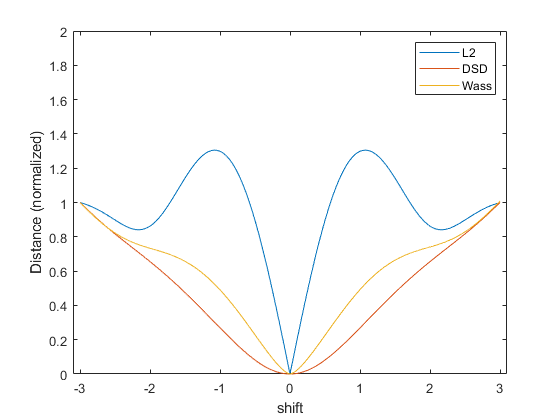
\includegraphics[width=2.8in]{Convex.png}
	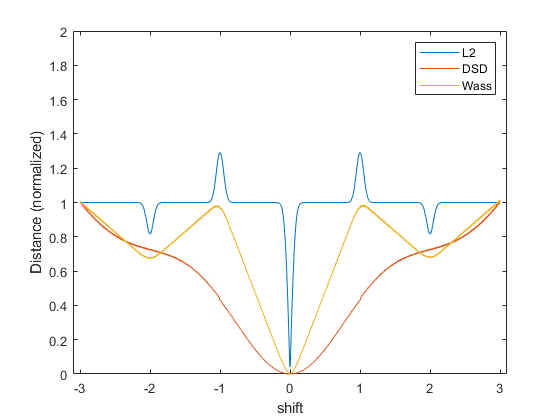
\includegraphics[width=2.8in]{Convex1.png}
	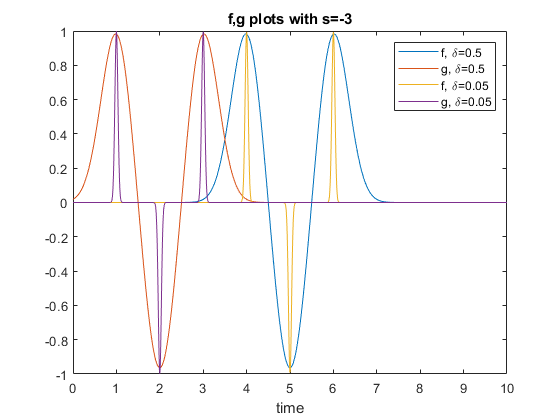
\includegraphics[width=2.8in]{fgplot.png}
	\caption{Plot of Convexity of DSD quasi-likelihood. Top plots normalized so when $s=-3$ the value on the plot is $1$. Left plot is for wide signals ($\delta = 0.5$) and right plot is for narrow signals ($\delta=0.05$).}
\end{figure}
Note that there are many ways to normalize the signals for the DSD quasi-likelihood and the Wasserstein quasi-likelihood. The option that has been used in this example is linear scaling, but other normalization protocols exist [1][7][8]. Linear scaling normalization is:

\hspace{\fill}$\widehat{\bm{f}}$=\Large$\frac{\bm{f}+c}{<\bm{f}+c>}$\normalsize \hspace{0.5cm}and \hspace{0.5cm}$\widehat{\bm{g}}$=\Large$\frac{\bm{g}+c}{<\bm{g}+c>}$, \vspace{0.5cm}\normalsize $<\bm{f}>=\sum_{i=1}^{N}f_i$\hspace{\fill} \normalsize (30)

Where $c$ is some constant chosen to ensure that both $\bm{f}+c>0$ and $\bm{g}+c>0$. The signals are then normalized to ensure that they can now be viewed as probability distributions. 
As seen in Figure 4.1, the DSD quasi-likelihood shows the best convexity for this specific example. The Gaussian likelihood produced many minima which, in a Bayesian inversion application, could produce an incorrect posterior. This example shows the advantage of using the DSD quasi-likelihood over the $L_2$ likelihood for inversion problems that involve phase shift. Note that it is possible to obtain better convexity from both DSD and Wasserstein quasi-likelihoods by choosing different ways of normalizing the initial signals $\bm{f}$ and $\bm{g}$.

\chapter{Numerical Algorithm}
In this section a Markov Chain Monte Carlo (MCMC) algorithm, along with the DSD quasi-likelihood, are used to create a numerical algorithm for the DSD Bayesian framework. The specific MCMC algorithm that will be used is the Metropolis-Hastings-within-Gibbs [9] (MH within G) sampling algorithm. MH within G is a method that combines two MCMC algorithms, the Gibbs sampler and Metropolis-Hastings sampler. The Gibbs sampler solves for the posterior of the hyper-parameter $s$, and the Metropolis-Hastings sampler solves for the posterior of the parameter vector $\bm{\theta}$. MH-within-G updates samples based on a selection process and keeps samples with a probability, $\alpha$ (see section 5.3). Looking at the posterior in Bayesian inversion, note that:
\begin{center}
	$\pi(\bm{\theta}|\bm{g}) \propto \pi(\bm{g}|\bm{\theta})\pi(\bm{\theta})$
\end{center}
This means that for a Bayesian algorithm we need a likelihood and prior. This is where we decide to use the DSD quasi-likelihood and employ a know algorithm, MH within G. 
\\
\section{\label{section:Gibbs Sampler}Gibbs Sampler}
Suppose that we have a gamma prior for $s$. That is, $s\sim Gamma(a,b)$, where $a,b>0$ are the shape and rate parameters of the Gamma prior. Employing this prior along with the DSD quasi-likelihood we have:
\begin{center}
	$\pi(s|\bm{\theta},\bm{g})\propto$ $\pi_{dsd}(\bm{g}|\bm{\theta},s)$ $\pi_{prior}(s)\propto se^{-sd_{dsd}}s^{a-1}e^{-bs}=s^{a}e^{-s(b+d_{dsd})}$
\end{center}
where $d_{dsd}=d_{dsd}(\bm{f}(\bm{\theta}$),$\bm{g})$. Note that the posterior is proportional to a Gamma distribution. To be exact:
\begin{center}
	$s\sim Gamma(a^*,b^*),$ \hspace{1cm} $a^*=a+1,$ \hspace{1cm}  $b^*=b+d_{dsd}$
\end{center}
This will be used to generate new values of $s$ with a given $\bm{\theta}$. Note that the prior here is a conjugate prior since both the prior and posterior of $s$ are Gamma distributions. This is not to say that the prior for $s$ must be a Gamma distribution. This is just the choice of prior for $s$ in this paper, and others may be used.
\section{\label{section:Metropolis-Hastings Sampler}Metropolis-Hastings Sampler}
The Gibbs sampler in the previous section assumes a fixed $\bm{\theta}$. The Metropolis-Hastings sampler [10][11] assumes a fixed $s$. Suppose then that we have a fixed value for $s$ and a posterior for $\bm{\theta}$.
\begin{center}
	$\pi(\bm{\theta}|s,\bm{g}) \propto \pi_{dsd}(\bm{g}|\bm{\theta},s)\pi_{prior}(\bm{\theta})$
\end{center}
Given a sample value of $\bm{\theta}$, call it $\bm{\theta^{(i)}}$, the goal is to generate a new sample, $\bm{\theta^{(i+1)}}$. Generate a candidate sample $\widetilde{\bm{\theta}}$ by sampling from a proposal distribution $q(\bm{\theta^{(i)}},\widetilde{\bm{\theta}})$ from the current sample $\bm{\theta^{(i)}}$.
\\ We then accept this candidate sample with probability [11]: \\

\hspace{\fill}$\alpha$=\Large$\frac{\pi(\widetilde{\bm{\theta}}|s,\bm{g})q(\bm{\theta^{(i)}},\widetilde{\bm{\theta}})}{\pi(\bm{\theta^{(i)}} |s,\bm{g})q(\widetilde{\bm{\theta}},\bm{\theta^{(i)}})}$=$\frac{\pi_{dsd}(\bm{g}|\widetilde{\bm{\theta}},s)\pi_{prior}(\widetilde{\bm{\theta}})q(\bm{\theta^{(i)}},\widetilde{\bm{\theta}})} {\pi_{dsd}(\bm{g}|\bm{\theta^{(i)}},s)\pi_{prior}(\bm{\theta^{(i)}})q(\widetilde{\bm{\theta}},\bm{\theta^{(i)}})}$\hspace{\fill} \normalsize (31)
\\ \\
This still leaves the choice of prior and proposal distributions. The choice of prior is often left up to experts for the specific problem since we want an expert to decide what we already know about the parameter $\bm{\theta}$. Sometimes nothing may be known about the prior distribution of $\bm{\theta}$. This is called a non-informative prior and would mean that $\pi_{prior}(\bm{\theta})=1$. As for the proposal distribution of $\widetilde{\bm{\theta}}$, a Gaussian random walk is often used and will be used in the examples in chapter 6:

\hspace{\fill}$\widetilde{\bm{\theta}} \sim Normal(\bm{\theta^{(i)}},\Sigma)$\hspace{\fill} \normalsize (32)

where $\Sigma$ is the covariance matrix. In the MH-within-G algorithm, the covariance matrix has a noticeable affect on the posterior and is often changed multiple times to see what works best for a given problem. Note here that if the proposal distribution is symetric (i.e. $q(\bm{\theta^{(i)}},\widetilde{\bm{\theta}})=q(\widetilde{\bm{\theta}},\bm{\theta^{(i)}})$), the terms with $q$ cancel out in the $\alpha$ ratio and we are left with [10]:
\begin{center}
	$\alpha=$\Large$\frac{\pi_{dsd}(\bm{g}|\widetilde{\bm{\theta}},s)\pi_{prior}(\widetilde{\bm{\theta}})} {\pi_{dsd}(\bm{g}|\bm{\theta^{(i)}},s)\pi_{prior}(\bm{\theta^{(i)}})}$
\end{center}
Symmetric proposals will be used in the examples in this paper so that this simplified $\alpha$ may be used. 
\newpage
\section{\label{section:Metropolis-Hastings-within-Gibbs}The Algorithm: Metropolis-Hastings-within-Gibbs in the DSD-Bayesian Framework}
$\bm{1.}$ \emph{Initialization}: Select an initial starting point $(\bm{\theta^{(0)}},s^{(0)})$ and set $i=0$.\\
$\bm{2.}$ \emph{Normalize}: Select a normalization protocol  to ensure that signals $\bm{f}$ and $\bm{g}$ are consistent with the definition of probability distributions. \\
$\bm{3.}$ \emph{Gibbs Sampler}: Generate $s^{(i+1)}$ from the posterior $\pi(s|\bm{\theta^{(i)}},\bm{g})$ with Gamma distribution
\begin{center}
	$s^{(i+1)}\sim Gamma(a^*,b^*)$, \hspace{1cm} $a^*=a+1$, \hspace{1cm} $b^*=b+d_{dsd}(\bm{f}(\bm{\theta^{(i)}}),\bm{g})$
\end{center}
$\bm{4.}$ \emph{Metropolis-Hastings Sampler}: Follow steps i-iii to generate $\bm{\theta^{(i+1)}}$:\\
\indent\indent i. Sample a candidate $\widetilde{\bm{\theta}}$ from the proposal distribution $q(\bm{\theta^{(i)}},\widetilde{\bm{\theta}})$\\
\indent\indent ii. Compute the ratio:
\begin{center}
		$\alpha(\bm{\theta^{(i)}},\widetilde{\bm{\theta}})$=\Large$\frac{\pi_{dsd}(\bm{g}|\widetilde{\bm{\theta}},s)\pi_{prior}(\widetilde{\bm{\theta}})q(\bm{\theta^{(i)}},\widetilde{\bm{\theta}})} {\pi_{dsd}(\bm{g}|\bm{\theta^{(i)}},s)\pi_{prior}(\bm{\theta^{(i)}})q(\widetilde{\bm{\theta}},\bm{\theta^{(i)}})}$
\end{center}
\indent\indent\indent iii. Set
\begin{center}
	$\bm{\theta^{(i+1)}}=\left\{
	\begin{array}{ll}
		\widetilde{\bm{\theta}}, & \quad Unif(0,1) \leq \alpha(\bm{\theta^{(i)}},\widetilde{\bm{\theta}}) \\
		\bm{\theta^{(i)}}, & \quad otherwise
	\end{array}
	\right.$
\end{center}
$\bm{5.}$ \emph{Iterate}: Increment $i$ by 1 and go to step 3.


\chapter{Numerical Examples from Seismic Inversion}
This section will explore several examples that implement the above DSD-Bayesian framework. These examples exist in the form of wave propagation, something seen in applications like seismic inversion. These examples serve to show the accuracy of this Bayesian framework and to compare it to both a Wasserstein framework and Gaussian framework. 
\section{\label{section:Problem Formulation}Problem Formulation}
All the examples in this section will use the same general one-dimensional source inversion problem. This problem is of similar form to an example in [1], allowing for a direct comparison to work in [1]. This problem has a wave pulse that propagates at a constant speed. The main  difference in each example will be the noise seen in the example. This will allow for direct comparison based on noise complexity as well as show the benefits of the DSD framework. \\\\

Suppose we have the Cauchy problem for the one-dimensional wave equation

\hspace{\fill}$u_{tt}(t,x)-u_{xx}(t,x)=0$, \hspace{1cm} $t\in [0,T]$, \hspace{1cm} $x\in \mathbb{R}$\hspace{\fill} \normalsize(33) 

\hspace{\fill}$u(0,x)=h(x;x_0,a)$, \hspace{1cm} $u_t(0,x)=0$\hspace{\fill} \normalsize (34)

With initial data

\hspace{\fill}$h(x;x_0,a)=a(e^{-100(x-x_0-0.5)^2}+e^{-100(x-x_0)^2}+e^{-100(x-x_0+0.5)^2})$\hspace{\fill} \normalsize (35)

This initial data acts as a source creating an initial wave pulse with given amplitude $a$ and initial starting location $x_0$. The solution to this problem is given by d'Alembert's formula [1]

\hspace{\fill}$u(t,x;x_0,a)=\frac{1}{2}h(x-t;x_0,a)+\frac{1}{2}h(x+t;x_0,a)$\hspace{\fill} \normalsize (36)

\section{\label{section:Example 1: Known Posterior}Example 1: Known Posterior}
This first example will show the accuracy of the DSD framework. Suppose that both the amplitude $a$ and initial position $x_0$ are treated as parameters in our Bayesian framework. That is to say that $\bm{\theta}=(\theta_1,\theta_2)$ where $\theta_1=x_0$ and $\theta_2=a$ are both unknown parameters. Suppose that we also have $N_r=7$ recievers each collectiong data located at $7$ different positions:
\begin{center}
	$x_1=-3$, $x_2=-2$, $x_3=-1$, $x_4=0$, $x_5=1$, $x_6=2$, $x_7=3$
\end{center}  
where each reciever is located at $x_r$ with $r=1,...,N_r$ and records noisy discrete-time data $g(t_k,x_r)$ over the time interval $[0,T]$ at $N$ discrete time levels $t_k=(k-1)\Delta t$ with $\Delta t=T/(N-1)$ and $k=1,...,N$. Let $f(t_k,x_r;\bm{\theta})$ be the corresponding simulated signal for a given $\bm{\theta}$ computed using $f(t_k,x_r;\bm{\theta})=u(t,x;\theta_1,\theta_2)$. Now, define the fixed parameter:
\begin{center}
	$\bm{\theta^*}=(\theta_1^*,\theta_2^*)$, \hspace{1cm}$\theta_1^*=0.1$, \hspace{1cm}$\theta_2^*=5$
\end{center}
and generate synthetic data $g(t_k,x_r)$ so that the posterior of $\bm{\theta}$ is known. This is done by first generating a true posterior distribution for $\bm{\theta}$.
\begin{center}
	$\pi_{posterior}(\theta_1|\bm{g})=Norm(\theta_1^*,0.001)$, \hspace{1cm} $\pi_{posterior}(\theta_2|\bm{g})=Norm(\theta_2^*,0.01)$
\end{center}
Define $\widehat{\theta_1}$ and $\widehat{\theta_2}$ so that:
\begin{center}
	$\widehat{\theta_1}\sim Norm(\theta_1^*,0.001)$ and $\widehat{\theta_2}\sim Norm(\theta_2^*,0.01)$
\end{center}
Now, sample values for $\widehat{\theta_1}$ and $\widehat{\theta_2}$ with $r=1,...,N_r$ and $k=1,...,N$ to produce 
\begin{center}
	$g(t_k,x_r)=f(t_k,x_r;\widehat{\theta_1}^{(rk)},\widehat{\theta_2}^{(rk)})$
\end{center}
where each $\widehat{\theta_1}^{(rk)}\sim Normal(\theta_1^*,0.001)$ and $\widehat{\theta_1}^{(rk)}\sim Normal(\theta_2^*,0.01)$. This allows us to test the accuracy of the DSD Bayesian framework since we can directly compare the results from the DSD framework to the true posteriors. Note that the data in this problem is two dimensional. This means that when storing the data $g(t_k,x_r)$ into a vector $\bm{g}$, we store it by defining

\begin{center}
 $\bm{g}=(g(t_1,x_1),g(t_2,x_1),...,g(t_N,x_1),g(t_1,x_2),g(t_2,x_2),...,g(t_N,x_2),...,g(t_N,x_{N_r}))$ 
 \end{center}
so that we translate the two dimensional data into a vector. This same procedure is done with $\bm{f}$. This means that vectors $\bm{f}$ and $\bm{g}$ have $n=N\times N_r$ entries.
\begin{figure}[H]
	\centering
	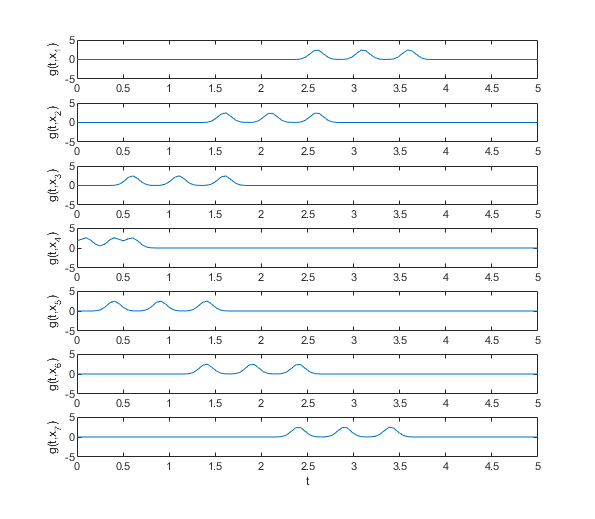
\includegraphics[width=4in,height=4in]{noiseData1.png}
    \caption{Observed signals with known posterior, recorded at seven receivers}
\end{figure}
\noindent Here are the following computations that were employed along with the DSD-Bayesian algorithm:\\
\indent $\bullet$\emph{Likelihood}: $\pi_{dsd}(\bm{g}|\bm{\theta})=s$[exp$(-sd_{dsd}(\bm{f}(\bm{\theta}),\bm{g}))$] (from equation 29)\\ \\
\indent $\bullet$\emph{Priors}: $\theta_1\sim Unif(-3,3)$, \hspace{0.5cm} $\theta_2\sim Unif(3,7)$, \hspace{0.5cm} $s\sim Gamma(1200,2)$ \\ \\
\overfullrule=0pt \indent $\bullet$\emph{Initial Data}: $\theta_1^{(0)}=0.6$, \hspace{0.5cm} $\theta_2^{(0)}=3$, \hspace{0.5cm} $s^{(0)}=70$\\\\
\indent $\bullet$\emph{Proposal}: $\widetilde{\bm{\theta}} \sim Normal(\bm{\theta^{(i)}},\Sigma)$ \indent with covariance matrix $\Sigma=diag(0.005,0.005)$.\\\\
Now, the DSD-Bayesian algorithm is ran with $M=500000$ iterations and remove the first $M_b=250000$ samples in the burn-in period. A thinning period of $M_t=4$ is used. That is to say that every $4^{th}$ is kept, and the rest are discarded. 
\begin{figure}[H]
	\centering
	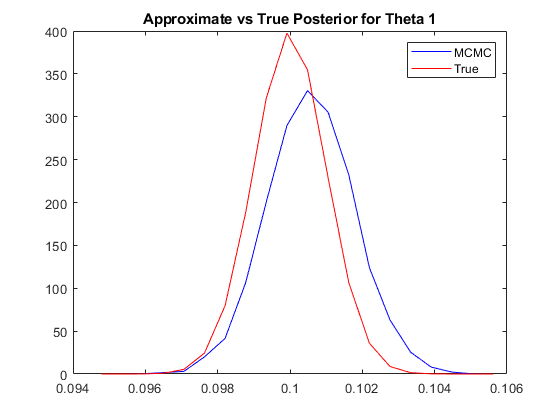
\includegraphics[width=2.5in,height=2in]{theta1.png}
	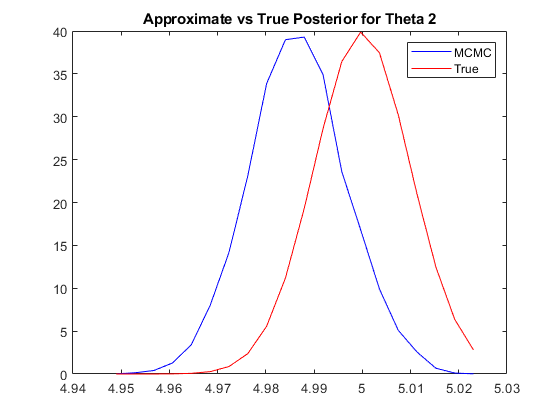
\includegraphics[width=2.5in,height=2in]{theta2.png}
	\caption{Approximate vs. true posteriors for $\theta_1$ and $\theta_2$. Appoximate posteriors found using DSD-Bayesian algorithm and are labeled MCMC (for Markov Chain Monte Carlo).}
\end{figure}
As seen in Figure 6.2, the approximate posterior converges to the true posterior. The error between the approximate and true posteriors can be measured using the Wasserstein distance, since this is a measure of dissimilarity between two probability distributions. The Wasserstein distance between the true and approximate posteriors for $\theta_1$ is $8.9198\times 10^{-4}$ and the Wasserstein distance between the true and approximate posteriors for $\theta_2$ is $1.446\times 10^{-2}$. Now, we can measure the Wassertein distance for different values of $M$ to get an idea about convergence. In Figure 6.3 we see how the Wasserstein distance between the true and approximate posteriors for $\theta_2$ decrease with a larger number of iterations, $M$. In Figure 6.3 a plot of $\mathcal{O}(1/M^2)$ is shown to give context to this convergence. \newpage
\begin{figure}[H]
	\centering
	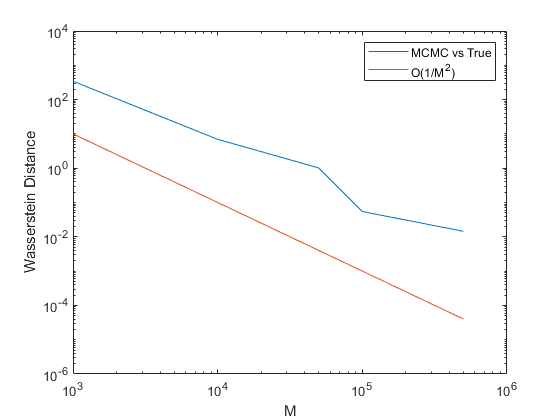
\includegraphics[width=3.8in,height=3in]{wassDist.png}
	\caption{Wasserstein distance for the approximate vs true posteriors of $\theta_2$ with varying number of iterations, $M$. MCMC solutions found using DSD-Bayesian framework.}
\end{figure}
\section{\label{section:Example 2: Additive Gaussian Noise with Unknown Phase and Amplitude}Example 2: Additive Gaussian Noise with Unknown Phase and Amplitude}
This example will compare the DSD framework to both the Wasserstein and Gaussian framework. This example will illustrate the advantage that optimal transport based Bayesian frameworks have over the standard Gaussian framework for problems involving additive Gaussian noise structures. Suppose that both amplitude $a$ and initial position $x_0$ are treated as parameters in our Bayesian framework. That is to say that $\bm{\theta}=(\theta_1,\theta_2)$ where $\theta_1=x_0$ and $\theta_2=a$ are both unknown parameters. Suppose we have $N_r=7$ receivers each collecting data located at 7 different positions:
\begin{center}
	$x_1=-3$, $x_2=-2$, $x_3=-1$, $x_4=0$, $x_5=1$, $x_6=2$, $x_7=3$
\end{center}
where each reciever is located at $x_r$ with $r=1,...,N_r$ and records noisy discrete-time data $g(t_k,x_r)$ over the time interval $[0,T]$ at $N$ discrete time levels $t_k=(k-1)\Delta t$ with $\Delta t=T/(N-1)$ and $k=1,...,N$. Let $f(t_k,x_r;\bm{\theta})$ be the corresponding simulated signal for a given $\bm{\theta}$ computed using $f(t_k,x_r;\bm{\theta})=u(t,x;\theta_1,\theta_2)$. Now, define the fixed parameter:
\begin{center}
	$\bm{\theta^*}=(\theta_1^*,\theta_2^*)$, \hspace{1cm} $\theta_1^*=0$, \hspace{1cm} $\theta_2^*=5$
\end{center}
and generate synthetic data $g(t_k,x_r)$ by polluting $f(t_k,x_r;\bm{\theta^*})$ with an additive Gaussian noise:
\begin{center}
	$g(t_k,x_r)=f(t_k,x_r;\bm{\theta^*})+\epsilon_{rk}$, \hspace{1cm} $\epsilon_{rk}\sim Normal(0,0.1)$
\end{center}
\begin{figure}[H]
	\centering
	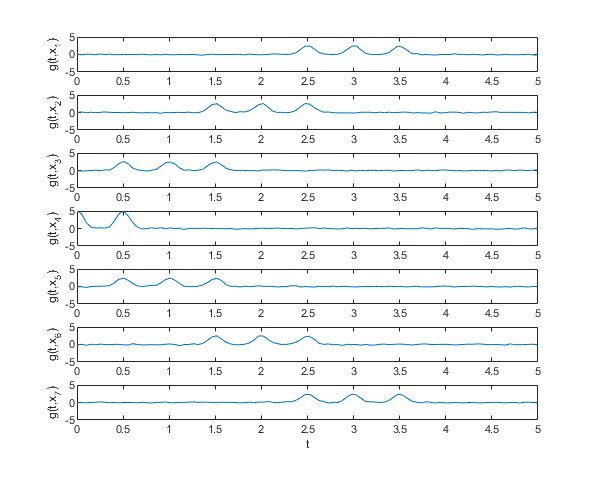
\includegraphics[width=4in,height=4in]{noiseData2.png}
	\caption{Observed signals with additive Gaussian noise, recorded at seven receivers}
\end{figure}
Here are the following computations that were employed along with the DSD-Bayesian algorithm:\\
\indent $\bullet$\emph{Likelihood}: $\pi_{dsd}(\bm{g}|\bm{\theta})=s$[exp$(-sd_{dsd}(\bm{f}(\bm{\theta}),\bm{g}))$] (from equation 29)\\ \\
\indent $\bullet$\emph{Priors}: $\theta_1\sim Unif(-3,3)$,  $\theta_2\sim Unif(3,7)$,  $s\sim Gamma(15000,0.3)$\\ \\
\overfullrule=0pt \indent $\bullet$\emph{Initial Data}: $\theta_1^{(0)}=0.6$, \hspace{0.5cm} $\theta_2^{(0)}=3$, \hspace{0.5cm} $s^{(0)}=70$, \hspace{0.5cm} \\\\
\indent $\bullet$\emph{Proposal}: $\widetilde{\bm{\theta}} \sim Normal(\bm{\theta^{(i)}},\Sigma)$ with covariance matrix $\Sigma=diag(0.00001,0.00001)$\\

\noindent Now, the DSD-Bayesian algorithm is ran with $M=50000$ iterations and remove the first $M_b=25000$ samples in the burn-in period. A thinning period of $M_t=2$ is used. That is to say that every $2^{nd}$ entry is kept, and the rest are discarded.
\begin{figure}[H]
	\centering
	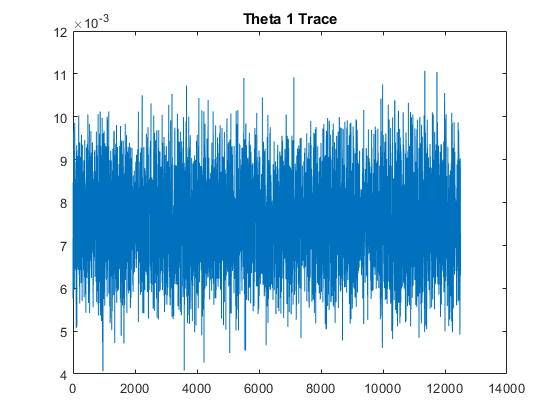
\includegraphics[width=2.5in,height=1.7in]{untitled1.png}
	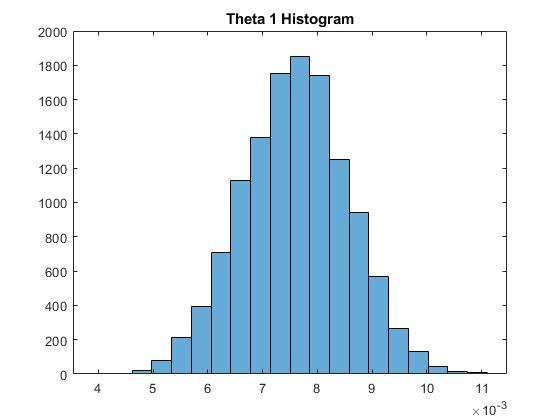
\includegraphics[width=2.5in,height=1.7in]{untitled2.png}
	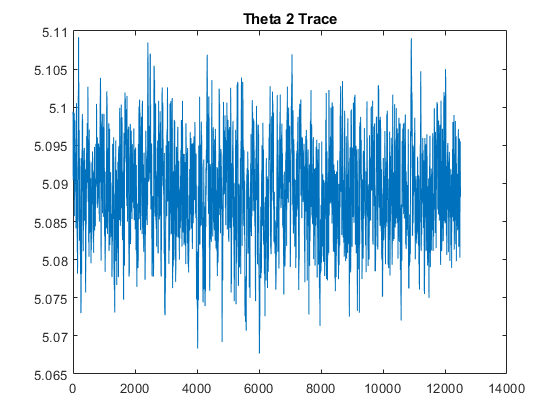
\includegraphics[width=2.5in,height=1.7in]{untitled3.png}
	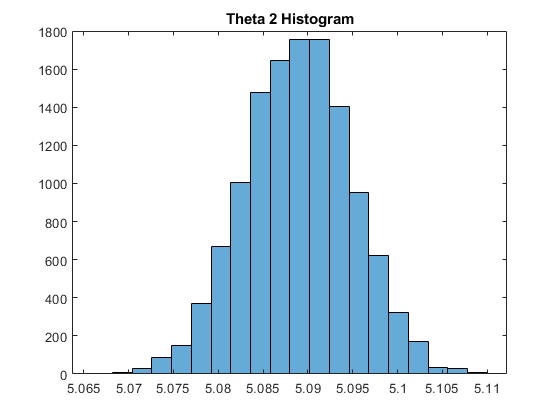
\includegraphics[width=2.5in,height=1.7in]{untitled4.png}
	\caption{Trace and Histograms for $\theta_1$ and $\theta_2$ found using DSD-Bayesian framework}
\end{figure}
\newpage \noindent  This same test is also ran using the Wasserstein quasi-likelihood and Gaussian likelihood (see figures 6.6 and 6.7). It is clear that the DSD and Wasserstein frameworks performed much better than the Gaussian framework. This is seen in the fact that the Gaussian framework produced posteriors that converge to incorrect values for $\theta_1$ and $\theta_2$. As stated in [1], the reason that this occurs is because the Gaussian framework produces many local minima, meaning that the Bayesian framework may fall into a false minimum and converge to an incorrect posterior. This is also what is seen in Figure 6.8 which shows that for this example the $L_2$ (or Gaussian) likelihood produces many extrema. 
\begin{figure}[H]
	\centering
	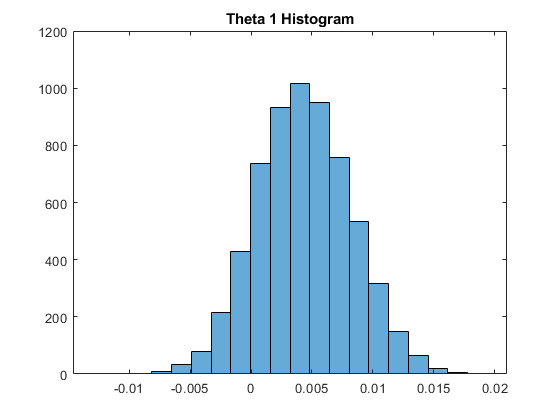
\includegraphics[width=2.7in,height=2in]{HistTheta1W.png}
	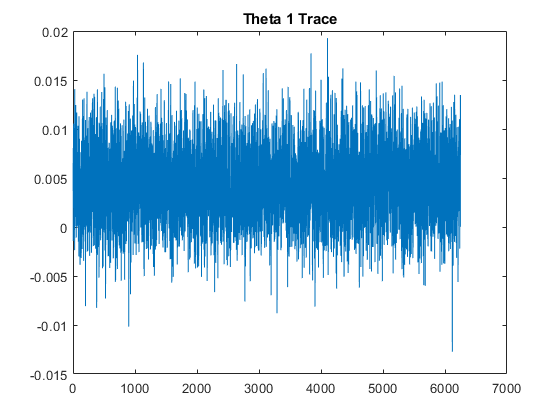
\includegraphics[width=2.7in,height=2in]{TraceTheta1W.png}
	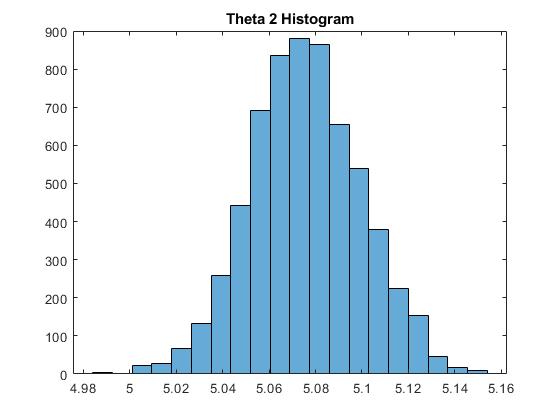
\includegraphics[width=2.7in,height=2in]{HistTheta2W.png}
	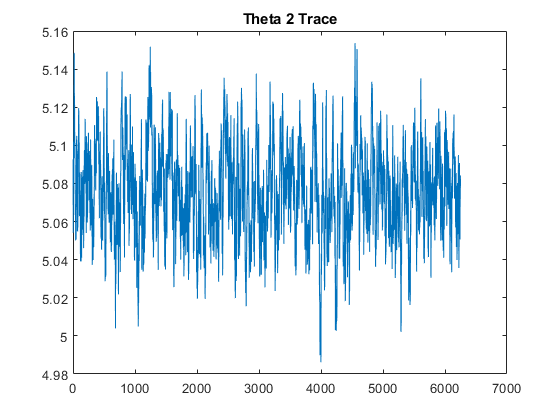
\includegraphics[width=2.7in,height=2in]{TraceTheta2W.png}
	\caption{Trace and Histograms for $\theta_1$ and $\theta_2$ found using Wasserstein-Bayesian framework. As seen in this figure as well as Figure 6.5, it is clear to see that the Wasserstein and DSD frameworks are converging to the same posterior because the histograms are centered at nearly the same values and the spread of these histograms are also similar.}
\end{figure}
\begin{figure}
	\centering
	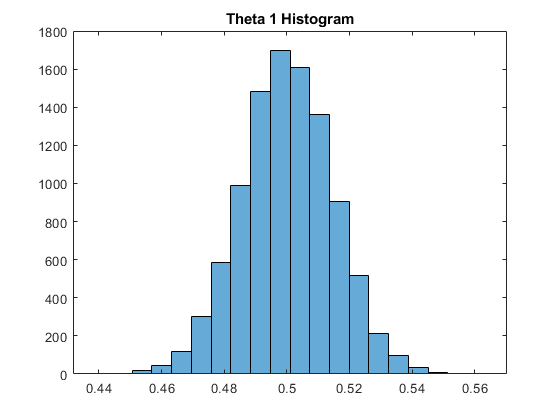
\includegraphics[width=2.7in,height=2in]{HistTheta1L2.png}
	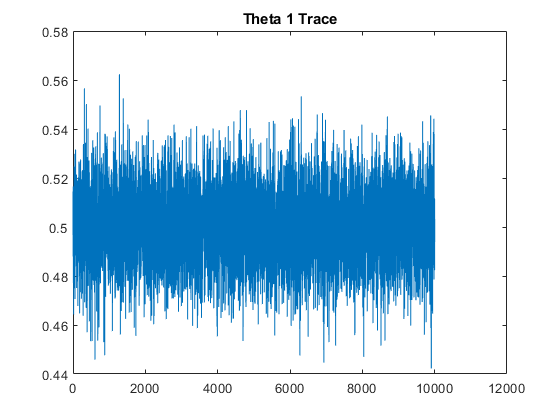
\includegraphics[width=2.7in,height=2in]{TraceTheta1L2.png}
	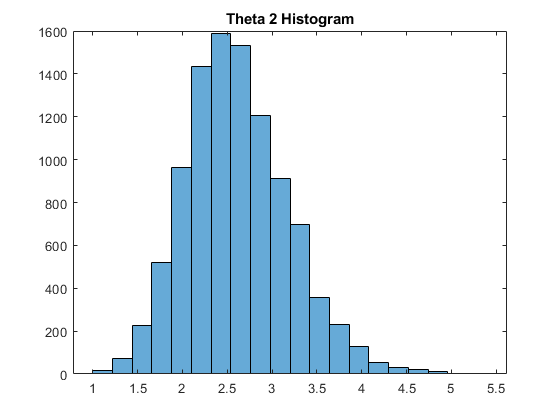
\includegraphics[width=2.7in,height=2in]{HistTheta2L2.png}
	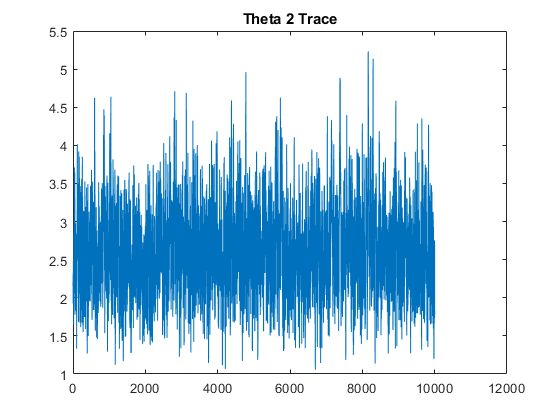
\includegraphics[width=2.7in,height=2in]{TraceTheta2L2.png}
	\caption{Trace and Histograms for $\theta_1$ and $\theta_2$ found using Gaussian-Bayesian framework. As clearly seen in the figures, the posteriors found from this Gaussian-Bayesian framework converged to incorrect values of $\theta_1$ and $\theta_2$.}
\end{figure}
\begin{figure}
	\centering
	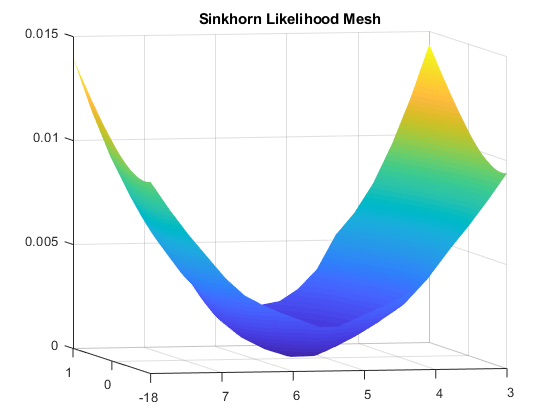
\includegraphics[width=2.7in,height=2in]{SinkMesh.png}
	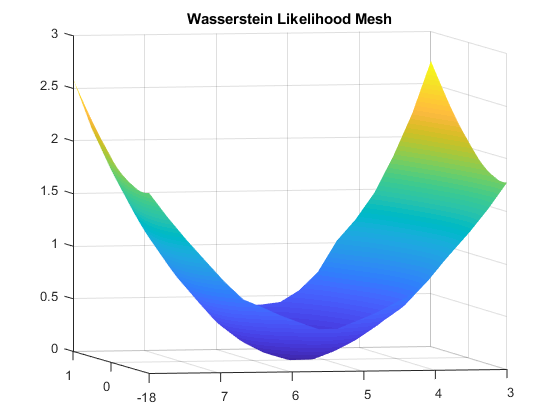
\includegraphics[width=2.7in,height=2in]{WassMesh.png}
	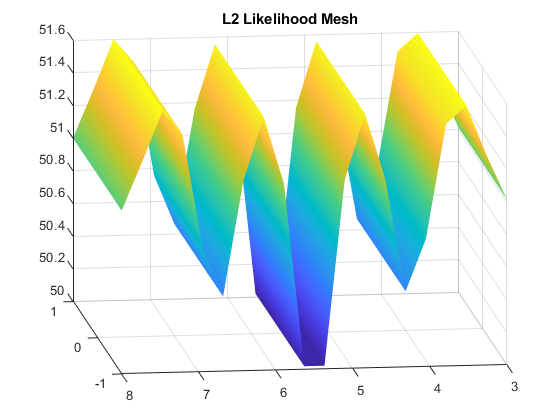
\includegraphics[width=2.7in,height=2in]{L2Mesh.png}
	\caption{Surface plots of DSD (left), Wasserstein (right), and $L_2$ (bottom) likelihoods for example 2. This shows that the $L_2$ likelihood did not stay convex and that the optimal transport quasi-likelihoods did.}
\end{figure}

\chapter{Conclusion}
Presented in this paper is a Bayesian framework based on Debiased Sinkhorn Divergence. This framework is based closely on the Wasserstein-Bayesian framework presented in [1], and preforms similarly in Example 2. The DSD-Bayesian framework allows for statistical independence, allowing for a more robust mathematical framework for Bayesian inversion for problems that do not involve statistical independence. This framework also has a computational time benefit over a higher dimensional Wasserstein framework, since Sinkhorn Divergence is a low cost regularized Wasserstein distance. This framework is well suited for inversion problems that involve phase shift, phase dilation, and amplitude change such as seismic events or other signal analysis problems. 


\chapter*{References}
\begin{enumerate}

	\item M. Motamed and D. Appelo. Wasserstein metric-driven Bayesian inversion with applications to signal processing. \emph{International J. for Uncertainty Quantification}, vol. 9, pp. 395-414, 2019.
	\item M. Motamed. Hierarchical low-rank approximation of regularized Wasserstein distance. 2020. https://arxiv.org/abs/2004.12511
	\item T. Bayes, R. Price, and J. Canton. An essay towards solving a problem in the doctrine
	of chances. By the late Rev. Mr. Bayes, F. R. S. communicated by Mr. Price, in a letter
	to John Canton, A. M. F. R. \emph{Philosophical Transactions of the Royal Society of London}, pages 370–418, 1763.
	\item Gut, Allan (2013). Probability: A Graduate Course (Second ed.). New York, NY: Springer. ISBN 978-1-4614-4707-8.
	\item J.-D. Benamou, B. D. Froese, and A. M. Oberman. Numerical solution of the Optimal
	Transportation problem using the Monge-Ampère equation. \emph{Journal of Computational
	Physics}, 260:107–126, 2014.
	\item B. Engquist, B.D. Froese Brittany, and Y. Yang. Optimal transport for seismic full
	waveform inversion. \emph{Communications in Mathematical Sciences}, 14(8):2309–2330, 2016.
	\item B. Engquist and Y. Yang. Seismic Imaging and Optimal Transport. \emph{To appear in Communications in Information and Systems, see also arXiv e-prints}, page arXiv:1808.04801, August 2018.
	\item L. Métivier, A. Allain, R. Brossier, Q. Mérigot, E. Oudet, and J. Virieux. Optimal transport for mitigating cycle skipping in full-waveform inversion: A graph-space transform
	approach. \emph{GEOPHYSICS}, 83(5):R515–R540, 2018.
	\item A. Gelman, J. B. Carlin, H. S. Stern, and D. B. Rubin. \emph{Bayesian data analysis}. Chapman
	and Hall/CRC, 2004.
	\item N. Metropolis, A. W. Rosenbluth, M. N. Rosenbluth, A. H. Teller, and E. Teller. Equation of state calculations by fast computing machines. \emph{The Journal of Chemical Physics},
	21:1087–1092, 1953
	\item S. Chib and E. Greenberg. Understanding the Metropolis-Hastings algorithm. The
	American Statistician, 49:327–335, 1995.
	\item C. Villani. Optimal Transport: Old and New, volume 338 of \emph{Grundlehren der mathematischen
	Wissenschaften}. Springer Verlag, 2009.
    \item C. Villani. Topics in Optimal Transportation, volume 58 of \emph{Graduate Studies in Mathematics}.
    American Mathematical Society, 2003.
    \item C. Villani. Optimal Transport: Old and New, volume 338 of \emph{Comprehensive Studies in
    Mathematics}. Springer-Verlag, Berlin, 2009.
	\item Y. Yang, B. Engquist, J. Sun, and B. F. Hamfeldt. Application of optimal transport
	and the quadratic Wasserstein metric to full-waveform inversion. \emph{Geophysics}, 83(1):R43–
	R62, 2018.
	\item M. Cuturi. Sinkhorn distances: Lightspeed computation of optimal transport. In \emph{Advances
	in Neural Information Processing Systems 26}, pages 2292–2300, 2013.
	\item G. Peyré and M. Cuturi. Computational optimal transport. \emph{Foundations and Trends in
	Machine Learning}, 11:355–607, 2019.
	\item J. Solomon, F. De Goes, G. Peyré, M. Cuturi, A. Butscher, A. Nguyen, T. Du, and L. Guibas.
	Convolutional Wasserstein distances: efficient optimal transportation on geometric domains.
	\emph{ACM Transactions on Graphics}, 34:66:1–66:11, 2015.
	\item A. Nemirovski and U. Rothblum. On complexity of matrix scaling. \emph{Linear Algebra and its
	Applications}, 302:435–460, 1999.
	\item B. Kalantari and L. Khachiyan. On the complexity of nonnegative-matrix scaling. \emph{Linear
	Algebra and its Applications}, 240:87–103, 1996.
	\item R. Sinkhorn. A relationship between arbitrary positive matrices and doubly stochastic matrices. \emph{Annals of Mathematical Statististics}, 35:876-879, 1964
	\item P.G. Bissiri, C.C. Holmes, and S.G. Walker. A General Framework for Updating Belief Distributions. \emph{Journal of the Royal Statistical Society, Statistical Methodology Series B}, 78:1103-1130, 2016.
	
\end{enumerate}



%\chapter{Derivation of $A = \pi r^2$}
%   A circle is really a square without corners.  QED.

%\bibliographystyle{AMS}
%\bibliography{bibfile_name}

\end{document}
